\mysubsubsection{Black-Box Testing}

%%%%%%%%%%%%%%%%%%%%%%%%%%%%%%%%%

\begin{frame}
\frametitle{Black Box vs. White Box Testing}
  % TODO: Translate image
  \begin{center}
  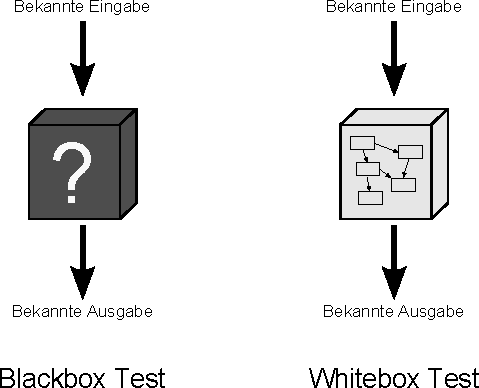
\includegraphics[width=.8\textwidth]{Qualitaetssicherung/abbildungen/BlackBoxAndWhiteBoxTesting}
  \end{center}
\end{frame}

%%%%%%%%%%%%%%%%%%%%%%%%%%%%%%%%%

\begin{frame}
\frametitle{Blackbox Testing of modules}
\begin{itemize}
  \item Idea: A part of a program is tested without looking at / knowing the code.
  \item Problem: How to define the test set? 
  \item Defining the test set can only rely on the specification.
  \item Systematic generation of test sets requires formal specification.
\end{itemize}
\end{frame}

%%%%%%%%%%%%%%%%%%%%%%%%%%%%%%%%%

\begin{frame}
\frametitle{Medieval Example}
Solutions for equations of the form:
\begin{equation*}
  x^3 + ax^2 + bx + c = 0
\end{equation*}
 
\begin{itemize}
  \item 1535: Tartaglia finds a solutions but keeps it to himself.
  \item Fior poses 30 problems to test this.
  \item See \citep{Wussing_Arnold1975}
\end{itemize}
\end{frame}

%%%%%%%%%%%%%%%%%%%%%%%%%%%%%%%%%

\begin{frame}
\frametitle{Medieval Black Box Text}
\setlength{\unitlength}{0.1\textwidth}
\begin{center}
\begin{picture}(9,5)
\put(0,5){\makebox(0,0)[tl]{Tartaglia}}
\put(9,5){\makebox(0,0)[tr]{Fior}}
\put(9,4){\makebox(0,0)[tr]{solves $(x-r)(x-s)(x-t)$}}
\put(4.5,3.3){\makebox(0,0){$x^3+ax^2+bx+c = 0$}}
\put(7,3){\vector(-1,0){5}}
\put(4.5,1.8){\makebox(0,0){r', s', t'}}
\put(2,1.5){\vector(1,0){5}}
\put(9,1){\makebox(0,0)[tr]{pr�ft $r=r', s=s', t=t'$}}
\end{picture}
\end{center}
\end{frame}


%%%%%%%%%%%%%%%%%%%%%%%%%%%%%%%%%
%
%\begin{frame}
%\frametitle{Blackbox Testing}
%\begin{center}
%\hspace*{4em} \pgfimage[width=0.8\textwidth]{Qualitaetssicherung/abbildungen/BlackboxTesten}
%\end{center}
%\end{frame}
%
%%%%%%%%%%%%%%%%%%%%%%%%%%%%%%%%%%
%
%\begin{frame}
%\frametitle{Example: Testing a parser}
%\underline{Idea:}
%\begin{center}
%\pgfimage[width=0.9\textwidth]{Qualitaetssicherung/abbildungen/Beispiel_Testen_eines_Parsers}
%\end{center}
%\end{frame}

%%%%%%%%%%%%%%%%%%%%%%%%%%%%%%%%%

\begin{frame}
\frametitle{Black Box Test methods}
\begin{itemize}
  \item Derive test cases from the program specification.
  \item Disregard program structure.
  \item Aim for comprehensive but avoid redundant testing of the functionality.
  \item Aim for functional coverage
  \item Defining a test case: 
    \begin{itemize}
      \item Build equivalence classes
      \item Test for extreme values
      \item Test special values
    \end{itemize}
\end{itemize}
\end{frame}

%%%%%%%%%%%%%%%%%%%%%%%%%%%%%%%%%

\begin{frame}
\frametitle{Equivalence Class Partitioning}
\structure{Aim}\\
Divide input and output parameter ranges into equivalence classes.
 
\vspace{\baselineskip}
\structure{Assumption}\\
A program reacts to any representative value from an equivalence class exactly like it reacts to all other members of the class.
 
\vspace{\baselineskip}
\structure{Representative value for a test case}\\
Pick any value from the class.
\end{frame}

%%%%%%%%%%%%%%%%%%%%%%%%%%%%%%%%%%

%\begin{frame}
%\frametitle{Building equivalence classes}
%\begin{center}
%\pgfimage[width=0.5\textwidth]{Qualitaetssicherung/abbildungen/Aequivalenzklassenbildung}
%\end{center}
%\end{frame}

%%%%%%%%%%%%%%%%%%%%%%%%%%%%%%%%%

\begin{frame}
\frametitle{Boundary Value Analysis}
\begin{itemize}
  \item Test cases that cover the boundary values of equivalence classes or that are in the vincinity of the boundaries uncover errors very often.
  \item Do not just pick any element from the equivalence class.
  \item Pick one or more elements such that every boundary of the equivalence class is tested.
\end{itemize}
\end{frame}

%%%%%%%%%%%%%%%%%%%%%%%%%%%%%%%%%

\begin{frame}
\frametitle{Equivalence classes with boundary values}
\begin{center}
\pgfimage[width=0.95\textwidth]{Qualitaetssicherung/abbildungen/AequivalenzklassenMitGrenzwerten}
\end{center}
\end{frame}

%%%%%%%%%%%%%%%%%%%%%%%%%%%%%%%%%

\begin{frame}
\frametitle{specification for a search function}
\begin{tabbing}
\hspace*{2em} \= \hspace{2em} \= \kill
\textbf{procedure} Search (Key : ELEM ; T: ELEM\_ARRAY;\\
\> Found : \textbf{in out} BOOLEAN; L: \textbf{in out} ELEM\_INDEX) ;\\[1 em]
\textbf{Pre-condition}\\
\> \> -- the array has at least one element\\
\> \> T'FIRST <= T'LAST\\
\textbf{Post-condition}\\
\> \> -- the element is found and is referenced by L\\
\> \> ( Found and T (L) = Key) \\
\> \> \textbf{or}\\
\> \> -- the element is not in the array\\
\> \> ( \textbf{not} Found \textbf{and} \\
\> \> \textbf{not} (\textbf{exists} i, T'FIRST >= i <= T'LAST, T (i) = Key ))
\end{tabbing}
\end{frame}

%%%%%%%%%%%%%%%%%%%%%%%%%%%%%%%%%

\begin{frame}
\frametitle{Building equivalence classes}
\framesubtitle{based on the specification}
\begin{itemize}
  \item Inputs that fulfil the pre-condition 
  \item Inputs that do not fulfil the pre-condition
  \item Inputs for which the key element is in the array
  \item Inputs for which the key element is not in the array
  \item Input sets
    \begin{itemize}
      \item With 0 elements
      \item Withe 1 element
      \item With multiple elements
    \end{itemize}
\end{itemize}
\end{frame}

%%%%%%%%%%%%%%%%%%%%%%%%%%%%%%%%%

\begin{frame}
\frametitle{Equivalence classes for the search function}
\begin{tabular}{l@{\hspace{2em}}l}\hline
\textbf{Array}      & \textbf{Element} \\ \hline 
Single value        & In sequence  \\ \hline   
Single value        & Not in sequence \\ \hline
More than 1 value   & First element in sequence \\ \hline
More than 1 value   & Last element in sequence  \\ \hline
More than 1 value   & Middle element in sequence \\ \hline
More than 1 value   & Not in sequence \\ \hline
\end{tabular}

\vspace{1em}
\begin{tabular}{l@{\hspace{2ex}}c@{\hspace{2ex}}l} \hline
\textbf{Input sequence} (T)  & \textbf{Key}  & \textbf{Output} (Found, L) \\ \hline
17                          & 17            & true, 1 \\ \hline
17                          & 0             & false, * \\ \hline
17, 29, 21, 23              & 17            & true, 1 \\ \hline
41, 18, 9, 31, 30, 16, 45   & 45            & true, 7 \\ \hline
17, 18, 21, 23, 29, 41, 38  & 23            & true, 4 \\ \hline
21, 23, 29, 33, 38          & 25            & false, * \\ \hline
\end{tabular}
\end{frame}

%%%%%%%%%%%%%%%%%%%%%%%%%%%%%%%%%

\begin{frame}
\frametitle{Black Box and White Box Testen}
  \begin{center}
  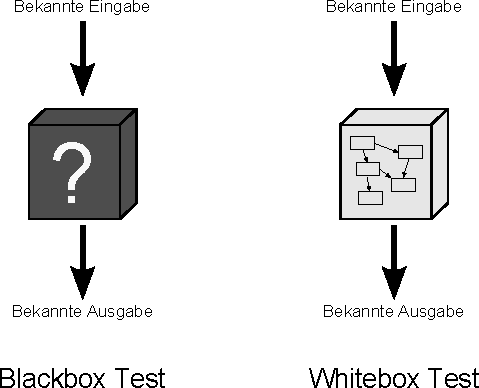
\includegraphics[width=.8\textwidth]{Qualitaetssicherung/abbildungen/BlackBoxAndWhiteBoxTesting}
  \end{center}
\end{frame}

%%%%%%%%%%%%%%%%%%%%%%%%%%%%%%%%%

\begin{frame}
\frametitle{Fuzzy Testing}
Fuzzing:
\begin{itemize}
	\item Unlike unit tests, fuzzy testing does not define test cases manually but generates them randomly based on statistic functions.
	\item By reaching a large number of generated tests, the software is tested for unusual values as well.
\begin{itemize}
	\item This is especially interesting for uncovering security relevant vulnerabilities.
\end{itemize}
\item Fuzzing is usually applied in black box testing to understand error affinity of new software and to detect vulnerabilities.
\item If a software reproducibly generates a problem (e.g. crashes) under fuzzy testing, white box tests can be used to find the exact cause. 
\end{itemize}
\end{frame}

%%%%%%%%%%%%%%%%%%%%%%%%%%%%%%%%%

\begin{frame}
\frametitle{Test Oracle}
  \begin{center}
  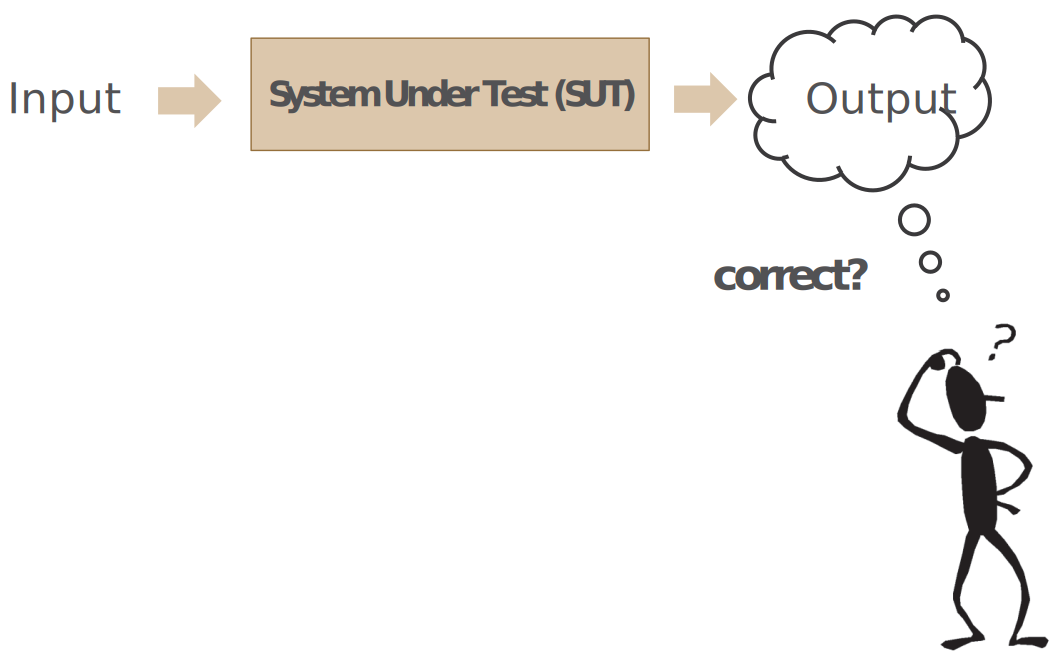
\includegraphics[width=\textwidth]{Qualitaetssicherung/abbildungen/TestOracle}
  \end{center}
\end{frame}

%%%%%%%%%%%%%%%%%%%%%%%%%%%%%%%%%

\begin{frame}
\frametitle{Are there classes of software that do not have a test oracle}
  \begin{center}
  \url{https://monti.com}  % unreachable
  \end{center}
\end{frame}

%%%%%%%%%%%%%%%%%%%%%%%%%%%%%%%%%

\begin{frame}
\frametitle{The oracle problem}
\framesubtitle{It is not always possible to define a test oracle}
  \begin{center}
\only<beamer>{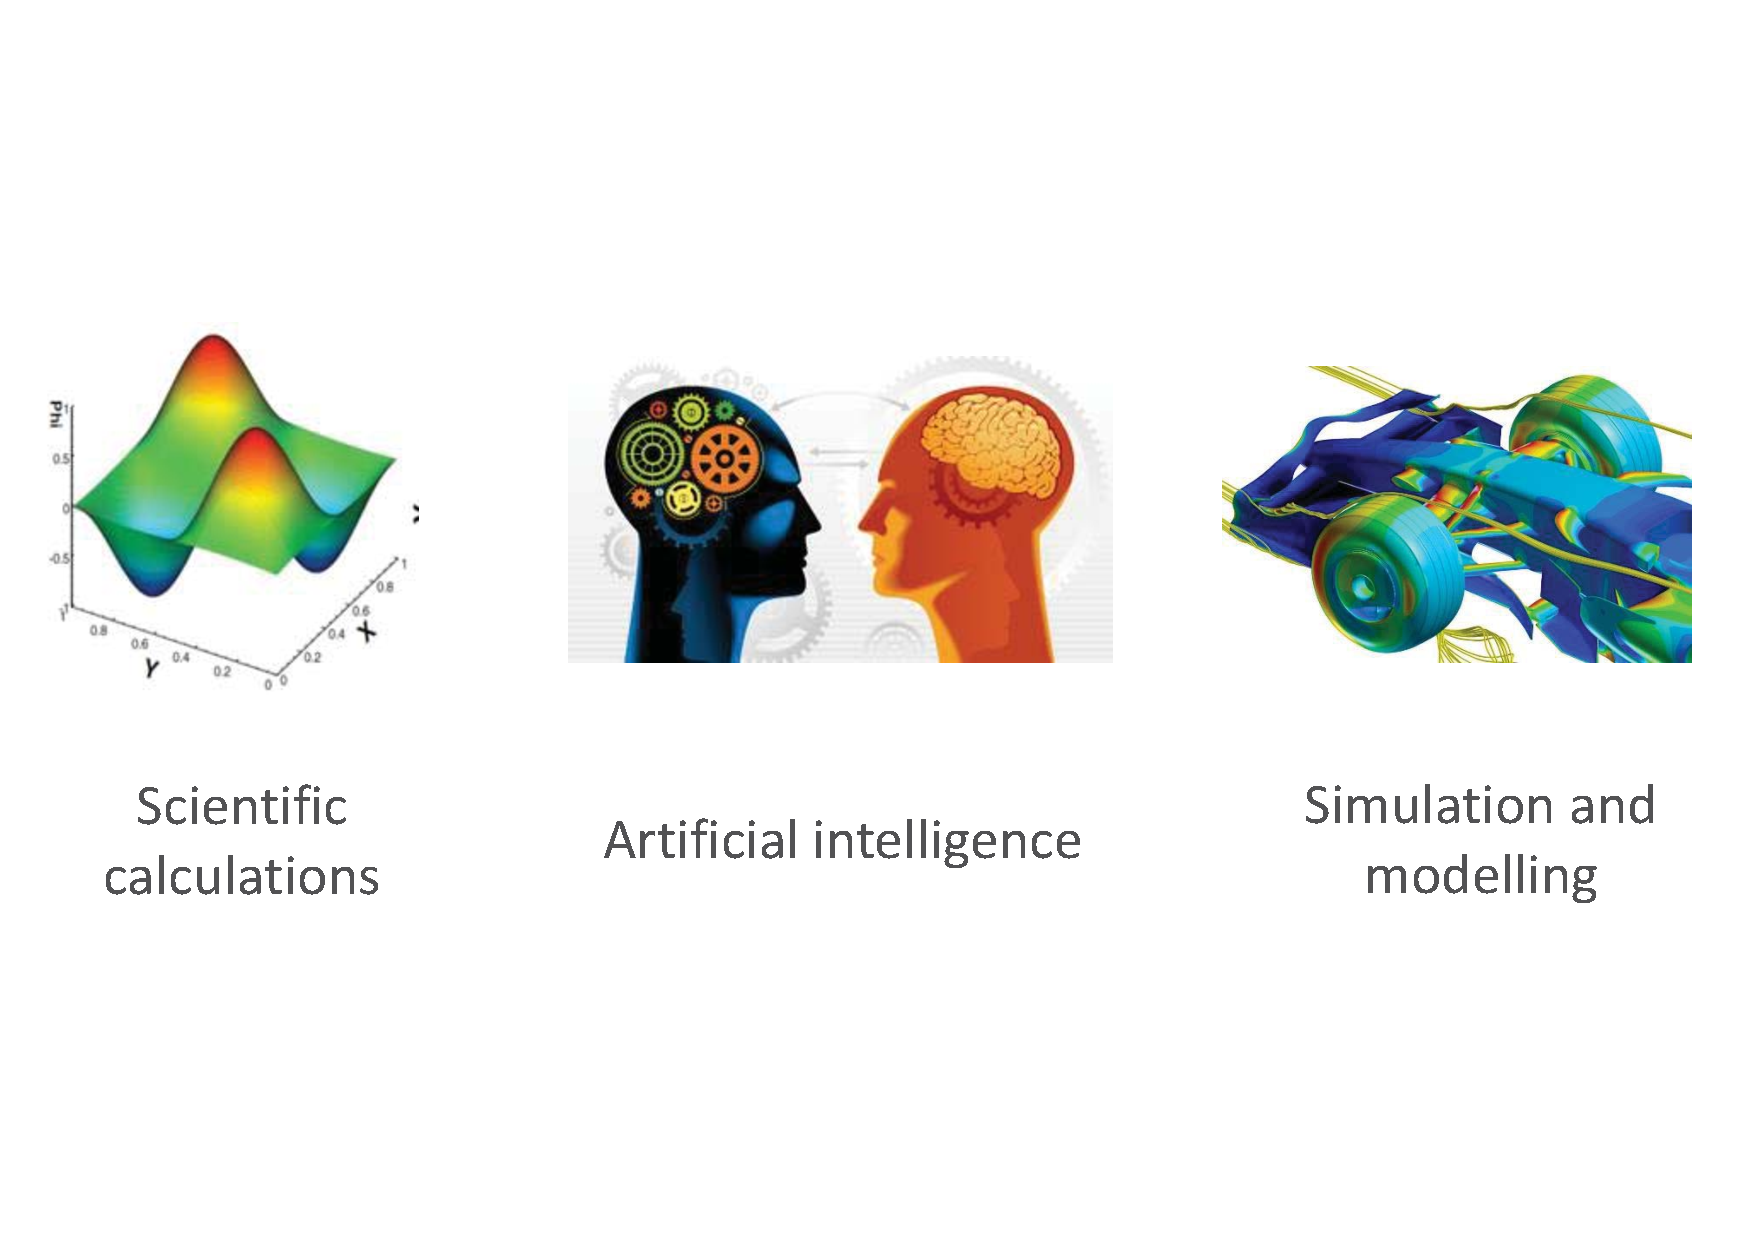
\includegraphics[width=\textwidth]{Qualitaetssicherung/abbildungen/TestOracleProblem}}
  \end{center}
	Was tun? \\
	\citet{MetamorphicTesting2016,segura_metamorphic_2020,kanewala_metamorphic_2019}
\end{frame}

%%%%%%%%%%%%%%%%%%%%%%%%%%%%%%%%%

\begin{frame}
\frametitle{Application of metamorphic testing}
\framesubtitle{\citet{segura_metamorphic_2020}}
  \begin{center}
\only<beamer>{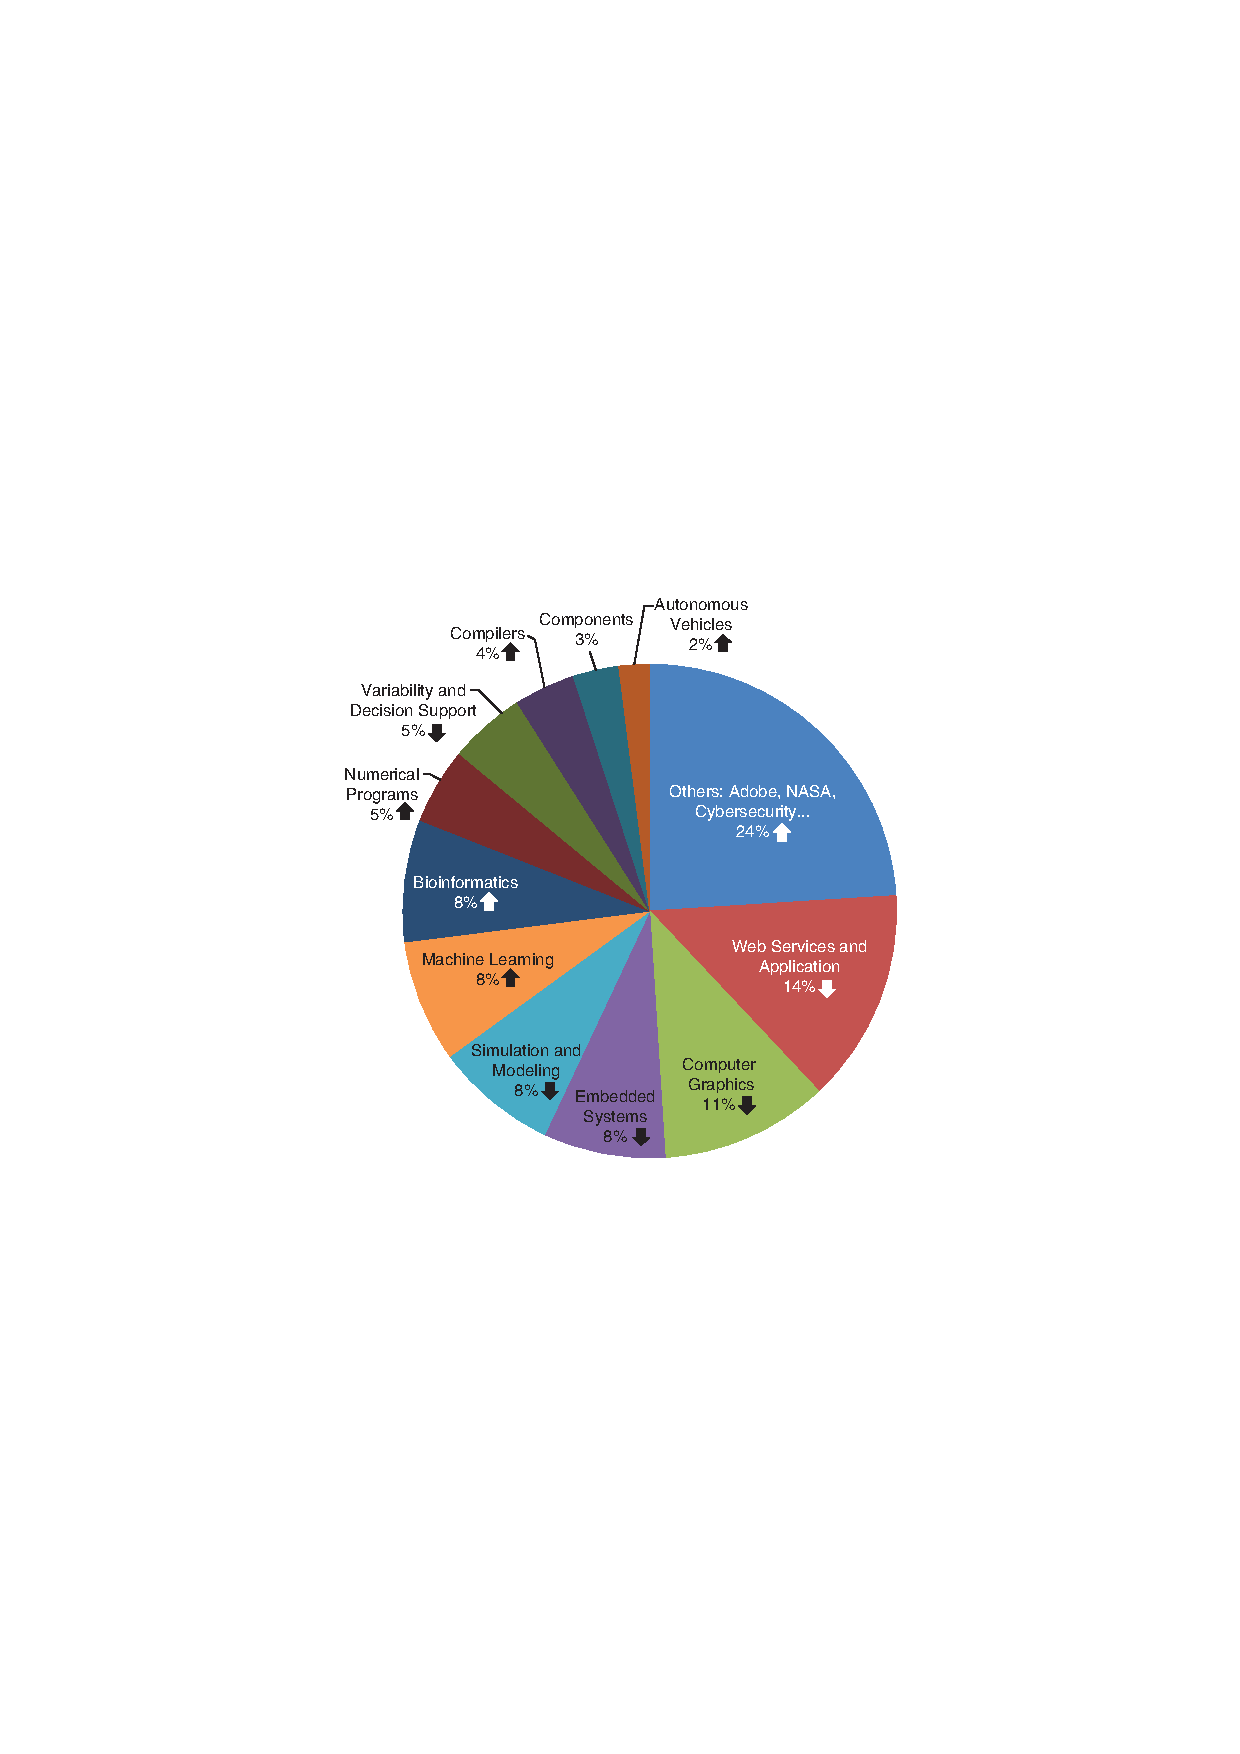
\includegraphics[width=.65\textwidth]{Qualitaetssicherung/abbildungen/MetamorphicTesting}}
  \end{center}
\end{frame}

